\documentclass{beamer}
\usepackage{tikz}
\usetikzlibrary{shapes}
\usetheme{Madrid}

\tikzstyle{rec} = [rectangle,draw,text centered,minimum width={width("Application")+2pt}]

\title[CSE 300: UIS]{CSE 300: Presentation of User Interface System}
\author[1605113]{Md. Zunaed Karim (1605113)}
\institute[BUET]{Bangladesh University of Engineering and Technology}
\date{\today}

\begin{document}
	
	\begin{frame}{A login application}
	\begin{figure}[h]
		\centering
		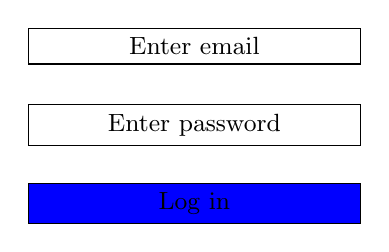
\begin{tikzpicture}
		[
		block/.style={
		draw,
		rectangle, 
		minimum width={width("Magnetometeraaaaaaaaaaa")+2pt},
		font=\small}
		]
		\node[block,fill=white](email) {Enter email};
		\node[block,fill=white,below of=email](password) {Enter password};
		\node[block,fill=blue,below of=password](login_button) {Log in};
		\end{tikzpicture}
	\end{figure}
	\end{frame}
	
	\begin{frame}{A login application}
	\begin{figure}[h]
		\centering
		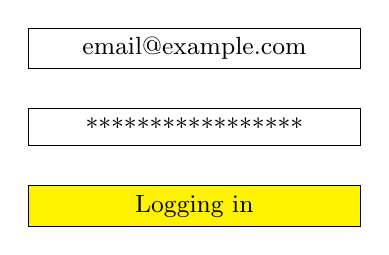
\begin{tikzpicture}
		[
		block/.style={
		draw,
		rectangle, 
		minimum width={width("Magnetometeraaaaaaaaaaa")+2pt},
		font=\small}
		]
		\node[block,fill=white](email) {email@example.com};
		\node[block,fill=white,below of=email](password) {*****************};
		\node[block,fill=yellow,below of=password](login_button) {Logging in};
		\end{tikzpicture}
	\end{figure}
	\end{frame}
	
	\begin{frame}{A login application}
	\begin{figure}[h]
		\centering
		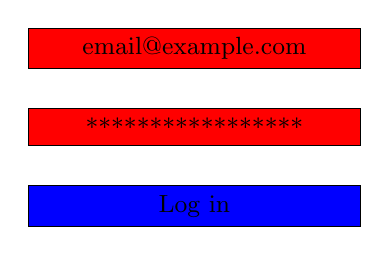
\begin{tikzpicture}
		[
		block/.style={
		draw,
		rectangle, 
		minimum width={width("Magnetometeraaaaaaaaaaa")+2pt},
		font=\small}
		]
		\node[block,fill=red](email) {email@example.com};
		\node[block,fill=red,below of=email](password) {*****************};
		\node[block,fill=blue,below of=password](login_button) {Log in};
		\end{tikzpicture}
	\end{figure}
	\end{frame}
	
	\begin{frame}{But what happens under the hood?}   	
   	\begin{figure}[h]
    	\centering
    	\begin{tikzpicture}
    	\node[rec,xshift=-1cm](Application) {Application};
    	\node[rec,right of=Application,xshift=2cm](UIS) {UIS};
    	\node[rec,right of=UIS,xshift=2cm](User) {User};\pause
    	
    	\draw[->] (Application.north) -- ++(0,2) -| (UIS);
    	\draw[->] (UIS.south) -- ++(0,-2) -| (User);
    	\draw[->] (User) -- (UIS);
    	\draw[->] (UIS) -- (Application);
    	  	
    	\end{tikzpicture}
    \end{figure}
	\end{frame}
	
	\begin{frame}{Building block of UIS}
	\begin{figure}[h]
		\centering
		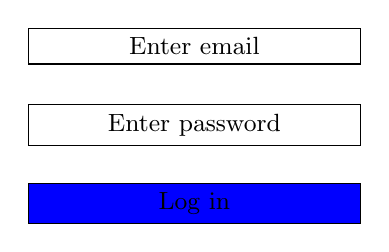
\begin{tikzpicture}
		[
		block/.style={
		draw,
		rectangle, 
		minimum width={width("Magnetometeraaaaaaaaaaa")+2pt},
		font=\small}
		]
		\node[block,fill=white](email) {Enter email};
		\node[block,fill=white,below of=email](password) {Enter password};
		\node[block,fill=blue,below of=password](login_button) {Log in};
		\end{tikzpicture}
	\end{figure}
	\end{frame}
	
	
	\begin{frame}{Building block of UIS}
	\begin{figure}[h]
		\centering
		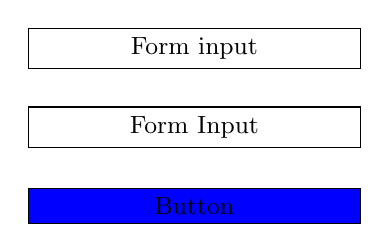
\begin{tikzpicture}
		[
		block/.style={
		draw,
		rectangle, 
		minimum width={width("Magnetometeraaaaaaaaaaa")+2pt},
		font=\small}
		]
		\node[block,fill=white](email) {Form input};
		\node[block,fill=white,below of=email](password) {Form Input};
		\node[block,fill=blue,below of=password](login_button) {Button};
		\end{tikzpicture}
	\end{figure}
	\end{frame}
	
	
	\begin{frame}{Building block of UIS}
	\begin{figure}[h]
		\centering
		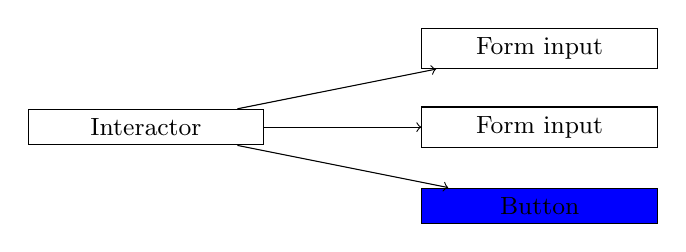
\begin{tikzpicture}
		[
		block/.style={
		draw,
		rectangle, 
		minimum width={width("Magnetometeraaaa")+2pt},
		font=\small}
		]
		\node[block,fill=white,xshift=8cm](email) {Form input};
		\node[block,fill=white,below of=email](password) {Form input};;
		\node[block,fill=white,left of=password,xshift=-4cm](interactor){Interactor};
		\node[block,fill=blue,below of=password](login_button) {Button};
		
    	\draw[->] (interactor) -- (email);
    	\draw[->] (interactor) -- (password);
    	\draw[->] (interactor) -- (login_button);
		\end{tikzpicture}
	\end{figure}
	\end{frame}
	
	
	\begin{frame}{But what happens under the hood?}   	
   	\begin{figure}[h]
    	\centering
    	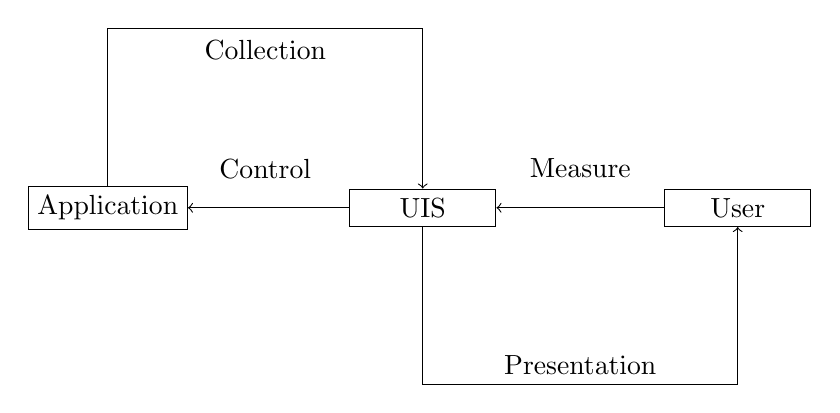
\begin{tikzpicture}
    	\node[rec,xshift=-1cm](Application) {Application};
    	\node[rec,right of=Application,xshift=3cm](UIS) {UIS};
    	\node[rec,right of=UIS,xshift=3cm](User) {User};\pause
    	
    	\draw[->] (User) -- (UIS);\pause
    	\draw[->] (UIS) -- (Application);\pause
    	\draw[->] (Application.north) -- ++(0,2) -| (UIS);\pause
    	\draw[->] (UIS.south) -- ++(0,-2) -| (User);\pause	
    	
    	
    	\node[xshift=5cm,yshift=.5cm](user_to_uis){Measure};
    	\node[xshift=1cm,yshift=.5cm](user_to_uis){Control};
    	\node[xshift=1cm,yshift=2cm](user_to_uis){Collection};
    	\node[xshift=5cm,yshift=-2cm](user_to_uis){Presentation};
    	  	
    	\end{tikzpicture}
    \end{figure}
	\end{frame}


	\begin{frame}{Modeling UIS with graphs}   	
   	\end{frame}

	
	\begin{frame}{Formal notations}   	
   	\end{frame}
		
	
	
\end{document}